\documentclass[a4paper,12pt]{article}
\usepackage[utf8]{inputenc}
\usepackage[T1]{fontenc}
\usepackage[english]{babel}
\usepackage{fullpage}
\usepackage{graphicx}
\usepackage{color}
\usepackage{listings}
\usepackage[scaled]{beramono}
\usepackage{subfig}
\usepackage{url}
\usepackage{hyperref}
\usepackage{nopageno}
\definecolor{bluekeywords}{rgb}{0.13,0.13,1}
\definecolor{greencomments}{rgb}{0,0.5,0}
\definecolor{redstrings}{rgb}{0.9,0,0}
\lstset{language=Bash,
	numbers=left,
	showspaces=false,
	showtabs=false,
	breaklines=true,
	showstringspaces=false,
	breakatwhitespace=true,
	escapeinside={(*@}{@*)},
	postbreak=\mbox{\textcolor{red}{$\hookrightarrow$}\space},
	commentstyle=\color{greencomments},
	keywordstyle=\color{bluekeywords}\bfseries,
	stringstyle=\color{redstrings},
	basicstyle=\ttfamily
}
\title{\vspace{-3em}%Projet 1A - BamboozLED\\
	
\includegraphics[width=.75\textwidth]{img/bamboozled2}}
\author{\textbf{Ludovic Blunat, Stanislas Bruhière and Renan Herniou}\\CentraleSupélec Rennes, academic year 2016/2017}
\date{}
\begin{document}
\maketitle
\begin{figure}[htbp]
	\centering
	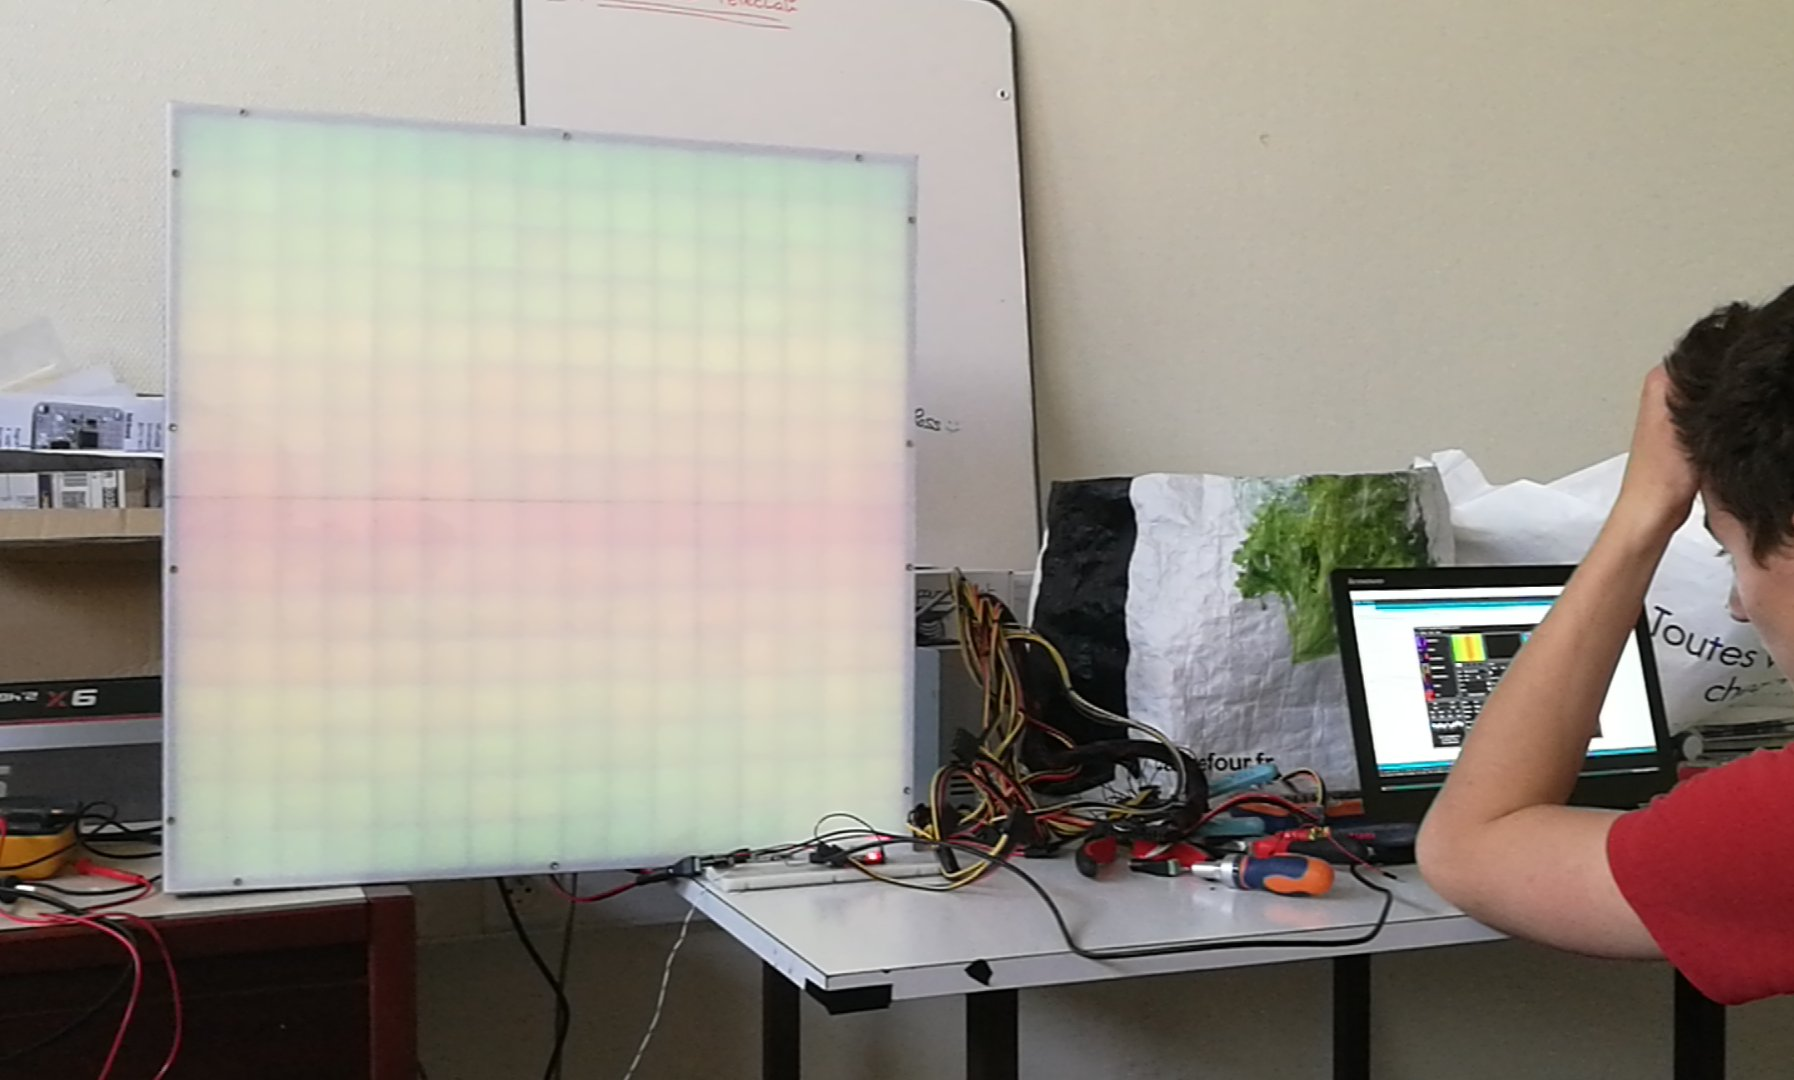
\includegraphics[width=\textwidth]{img/cover}
\end{figure}\newpage
\section{How does addressable LEDs work?}
First of all, we focus on the behavior of an addressable LED strip such as the one used in this project (with WS2812 RGB LEDs). Why such a component? Because it is cheap and available in several configurations (LEDs density, waterproof or not, etc.). Strips used in this project \cite{led} have 3 pins: ground, 5V and a data pin.
\begin{figure}[htbp]
\centering
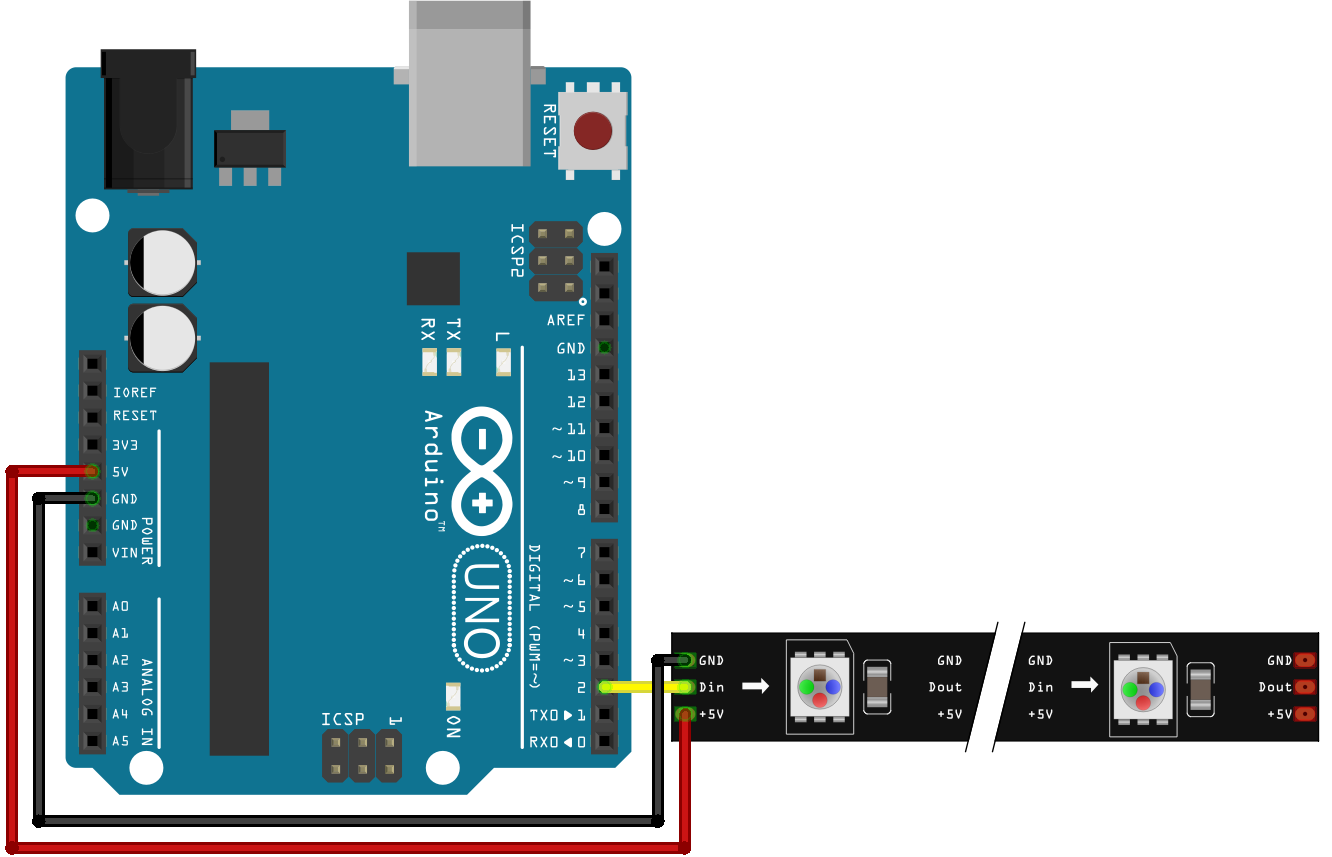
\includegraphics[height=.3\textheight]{img/led_strip}
\end{figure}\\
A single strip is connected to an Arduino board which sends 8-bit RGB and intensity values. Fortunately for us, we do not have to dive at the register level to control such a component: Adafruit has published a library online: \url{https://github.com/adafruit/Adafruit_NeoPixel}.\\

Each WS2812 LED includes a microcontroller processing the data signal; first 3 bytes are taken into account by the LED cell; then, the microcontroller sends remaining bytes to the next LED. Each WS2812 can be seperated from others; furthermore, we can solder power/signal pins to create a custom layout without breaking the transmission between all LEDs.\\

An LED is an optoelectronic component: it is able to produce light when powered by an electric current. Unlike incandescent light bulbs, an LED does not contain a filament but several semiconductors layers. These semiconductors (aluminium nitride $AlN$ and gallium phosphate $GaPO_4$) do not create current resistance nor energy loss when emitting light.\\

When an electric current crosses semiconductor layers, many electrons encounter positively charged atoms creating energy as a light flux. The light flux is nearly monochromatic due to a small transmission bandwidth. We can play with the light wavelength by modifying semiconductor layers. Several semiconductor technologies are available on the market. A RGB LED consists of 3 seperate cells emitting at 3 wavelengths (for red, green and blue). The microcontroller embedded in the WS2812 chip adjusts the voltage for each monochromatic cell in order to vary the intensity and the overall color emitted by the WS2812.
\begin{figure}[htbp]
	\centering
	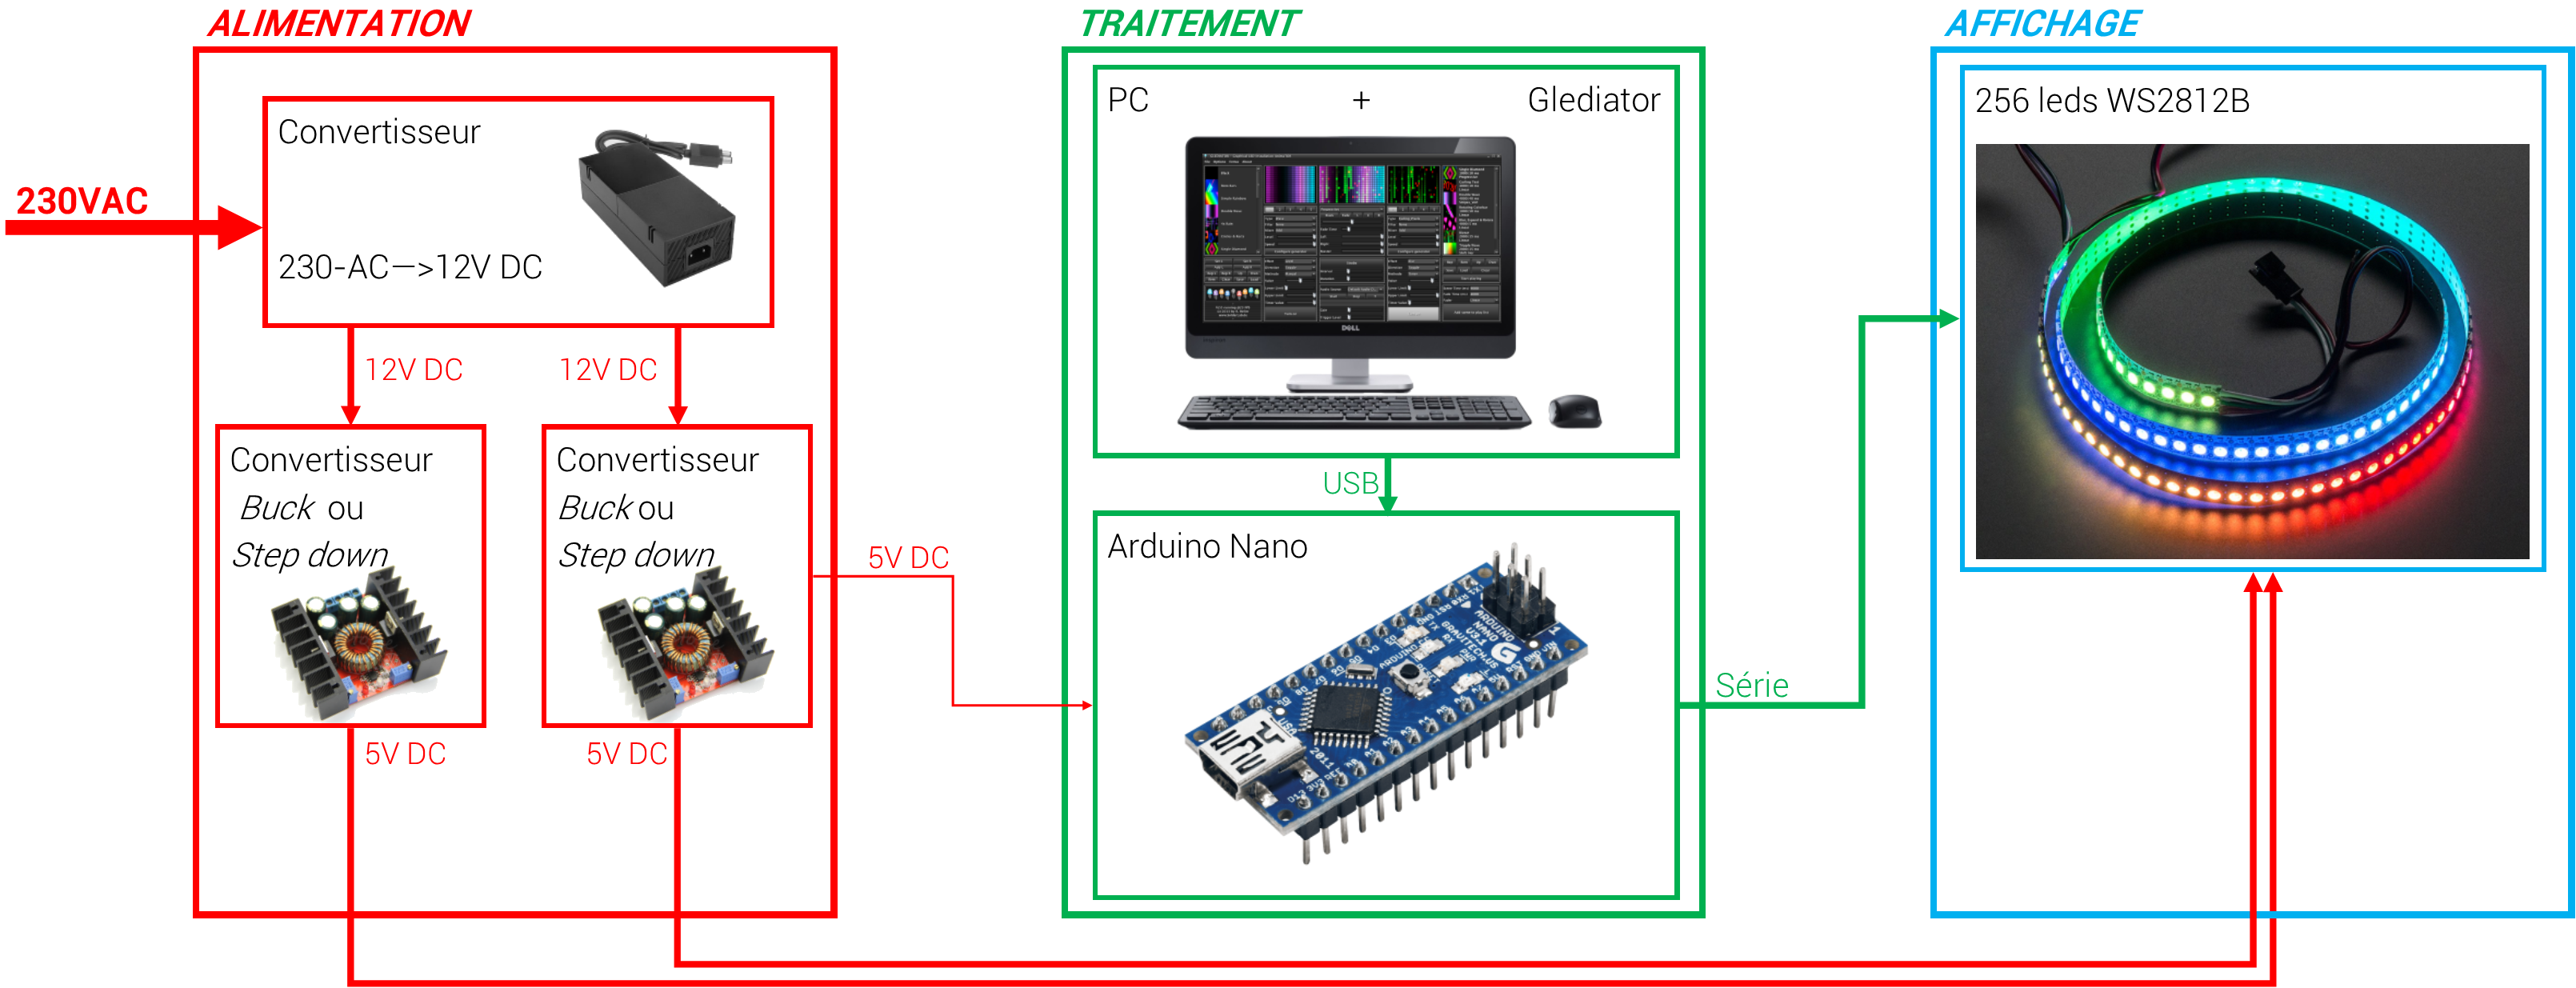
\includegraphics[width=\textwidth]{img/global}
\end{figure}
\section{Project description}
We have built a 16x16 LED panel which can be controlled by an Arduino. Each LED can be controlled individually: therefore, we are able to create animations on the panel.

\subsection{Power supply}
In such a project, the power supply is not the easiest part: in fact, during our first test phasis, we have seen that current consumption was quite high. After several searches, it turns out that the maximum current by a RGB LED is about 60 mA (20mA for each subpixel). In the worst case (each pixel transmitting a white light at maximum brightness), BamboozLED\textsuperscript{TM} could consume up to 255*0.05=15.36A!
\begin{itemize}
\item First, we thought to use a computer power supply: unfortunately, it did not deliver enough current and turned off into a secured mode before it shut down. BamboozLED\textsuperscript{TM} was bamboozled :|
\item Then, we looked for 5V power supply: however, 5V with high current features are \textbf{really} rare. In other words, it was nearly impossible to find it\ldots
\end{itemize}
Finally, we chose a 12V power supply. We needed to lower the input voltage to 5V using a Buck boost converter \cite{laomao,salar}. However, such converters rarely deliver more than 10A. The trick consisted in dividing the LED panel in two parts: each part has its own Buck boost converter.

\subsection{Structure}
The frame of BamboozLED\textsuperscript{TM} is made of 10mm-wide wood panels, its whole size is a parallelepipoid of 540*540*30mm.
\begin{figure}[htbp]
	\centering
	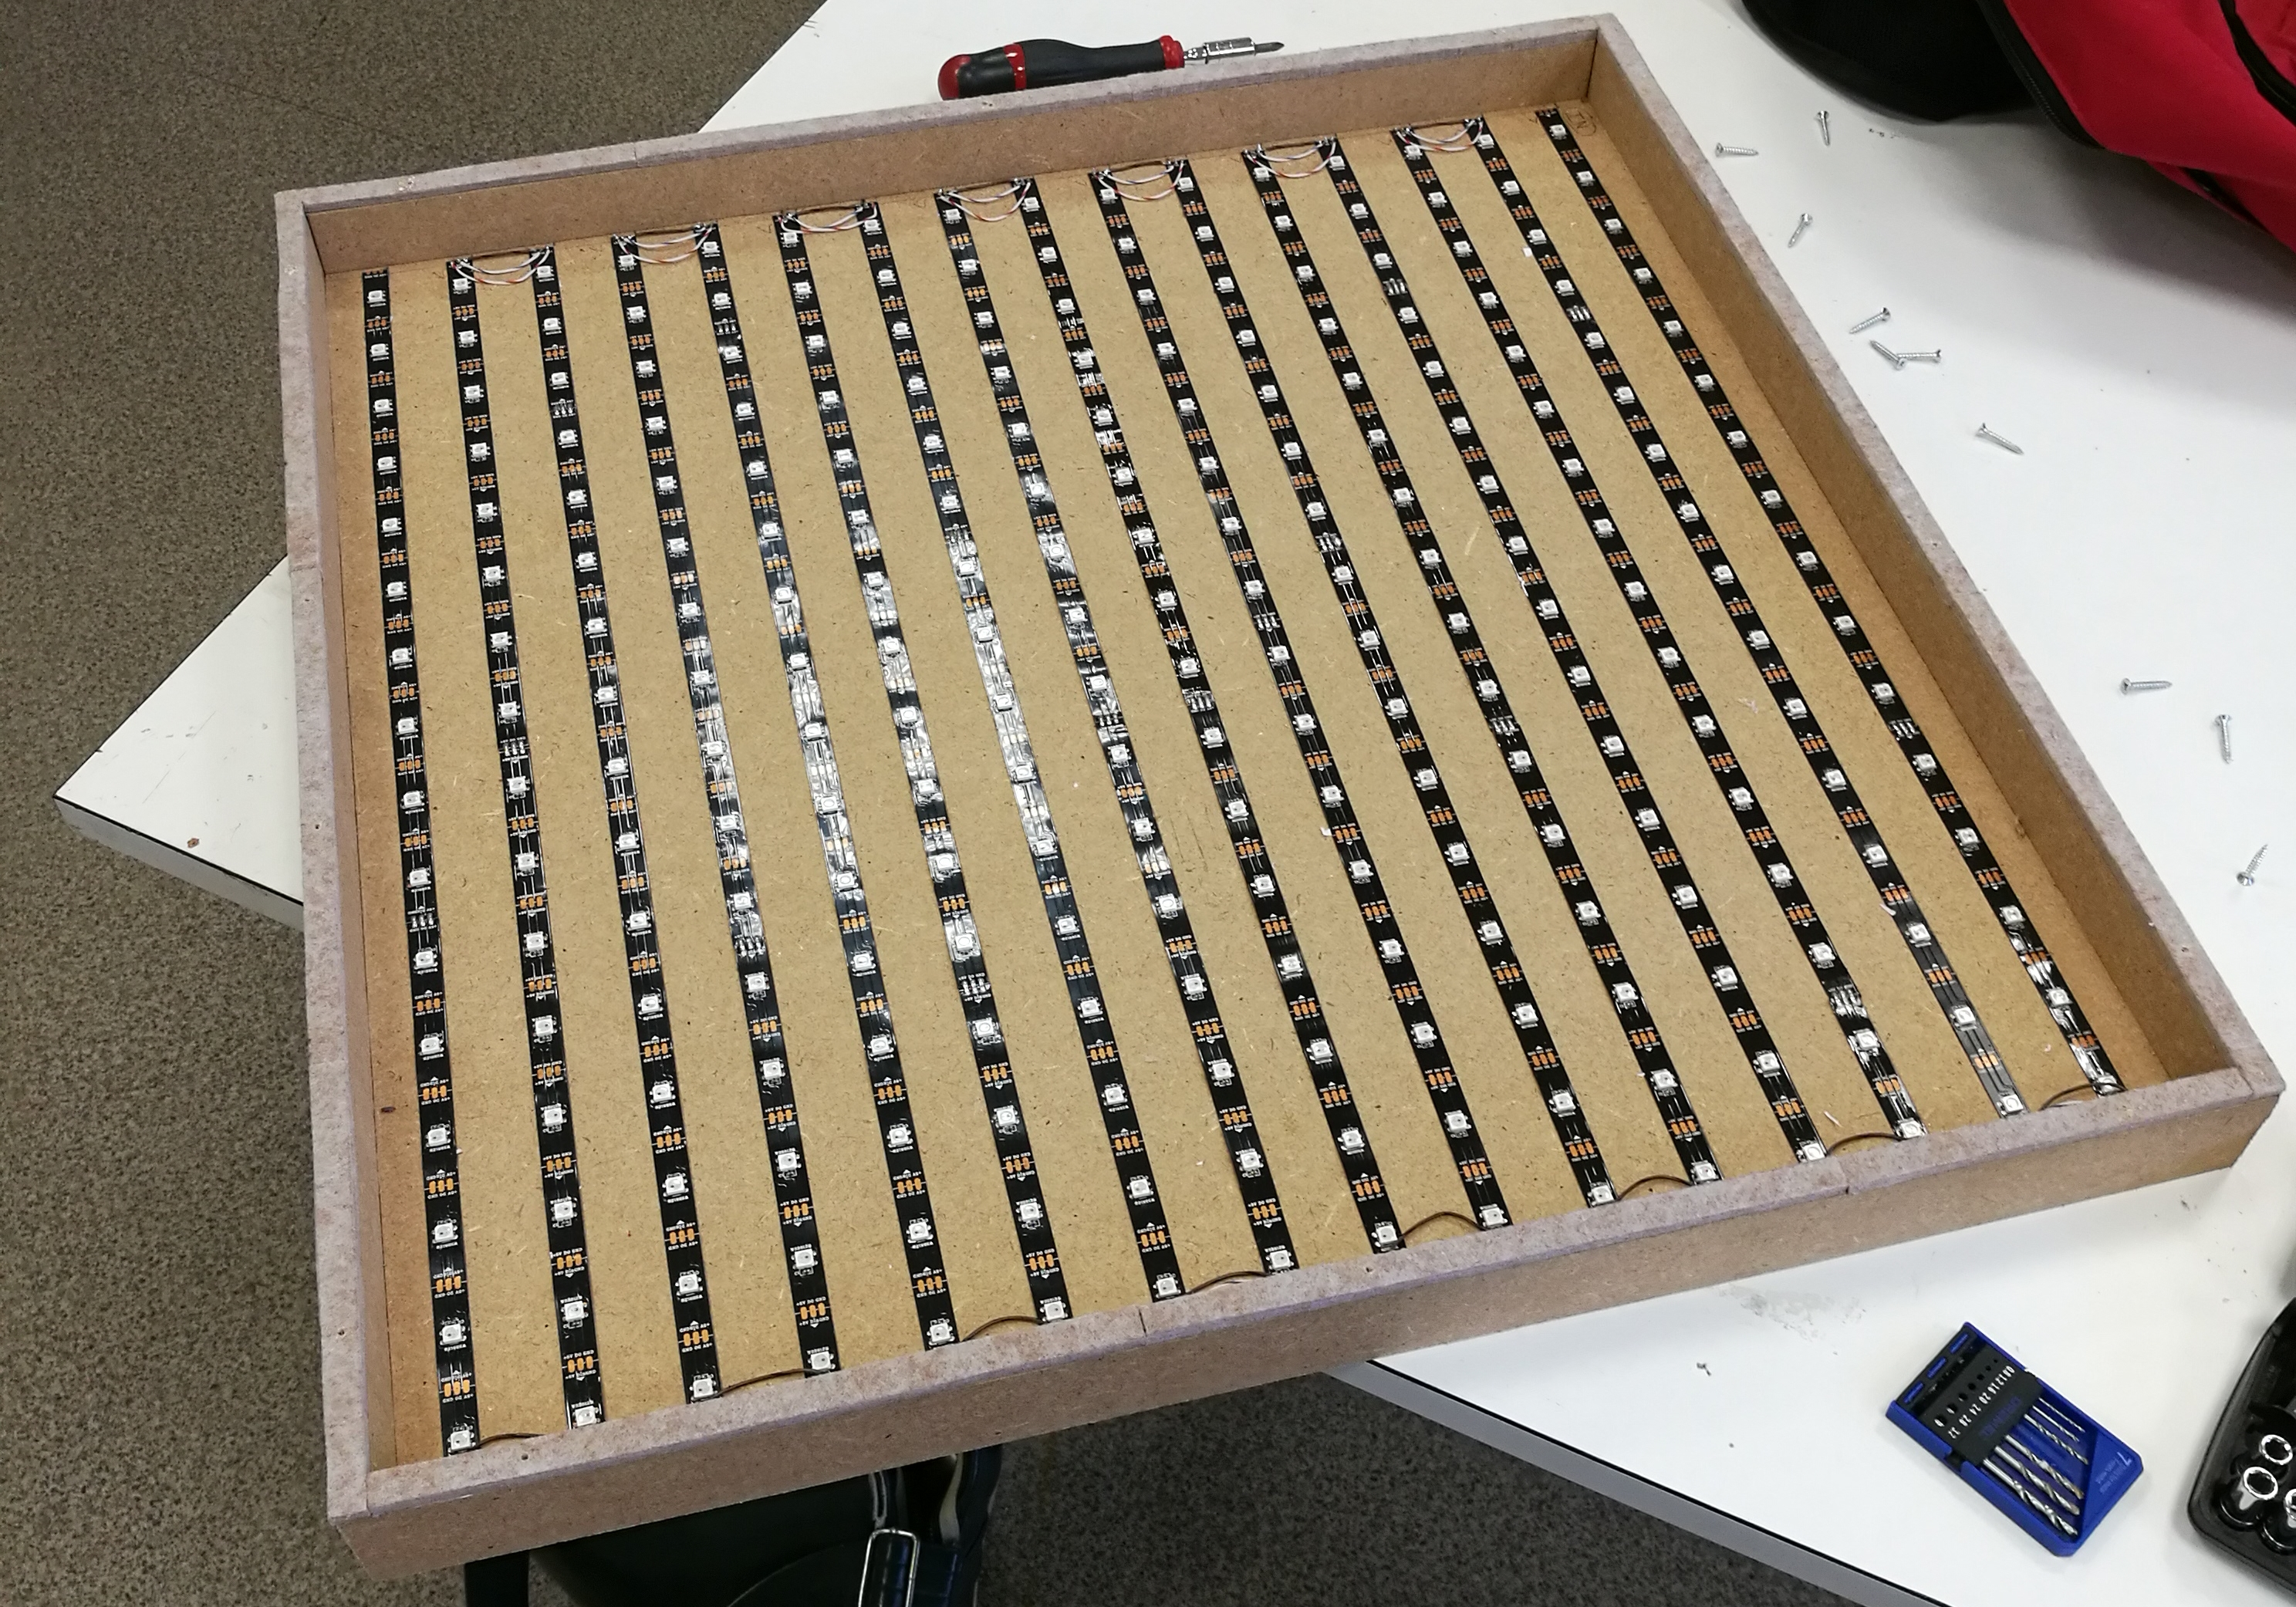
\includegraphics[width=\textwidth]{img/pic1}
\end{figure}\\
\begin{figure}[htbp]
	\centering
	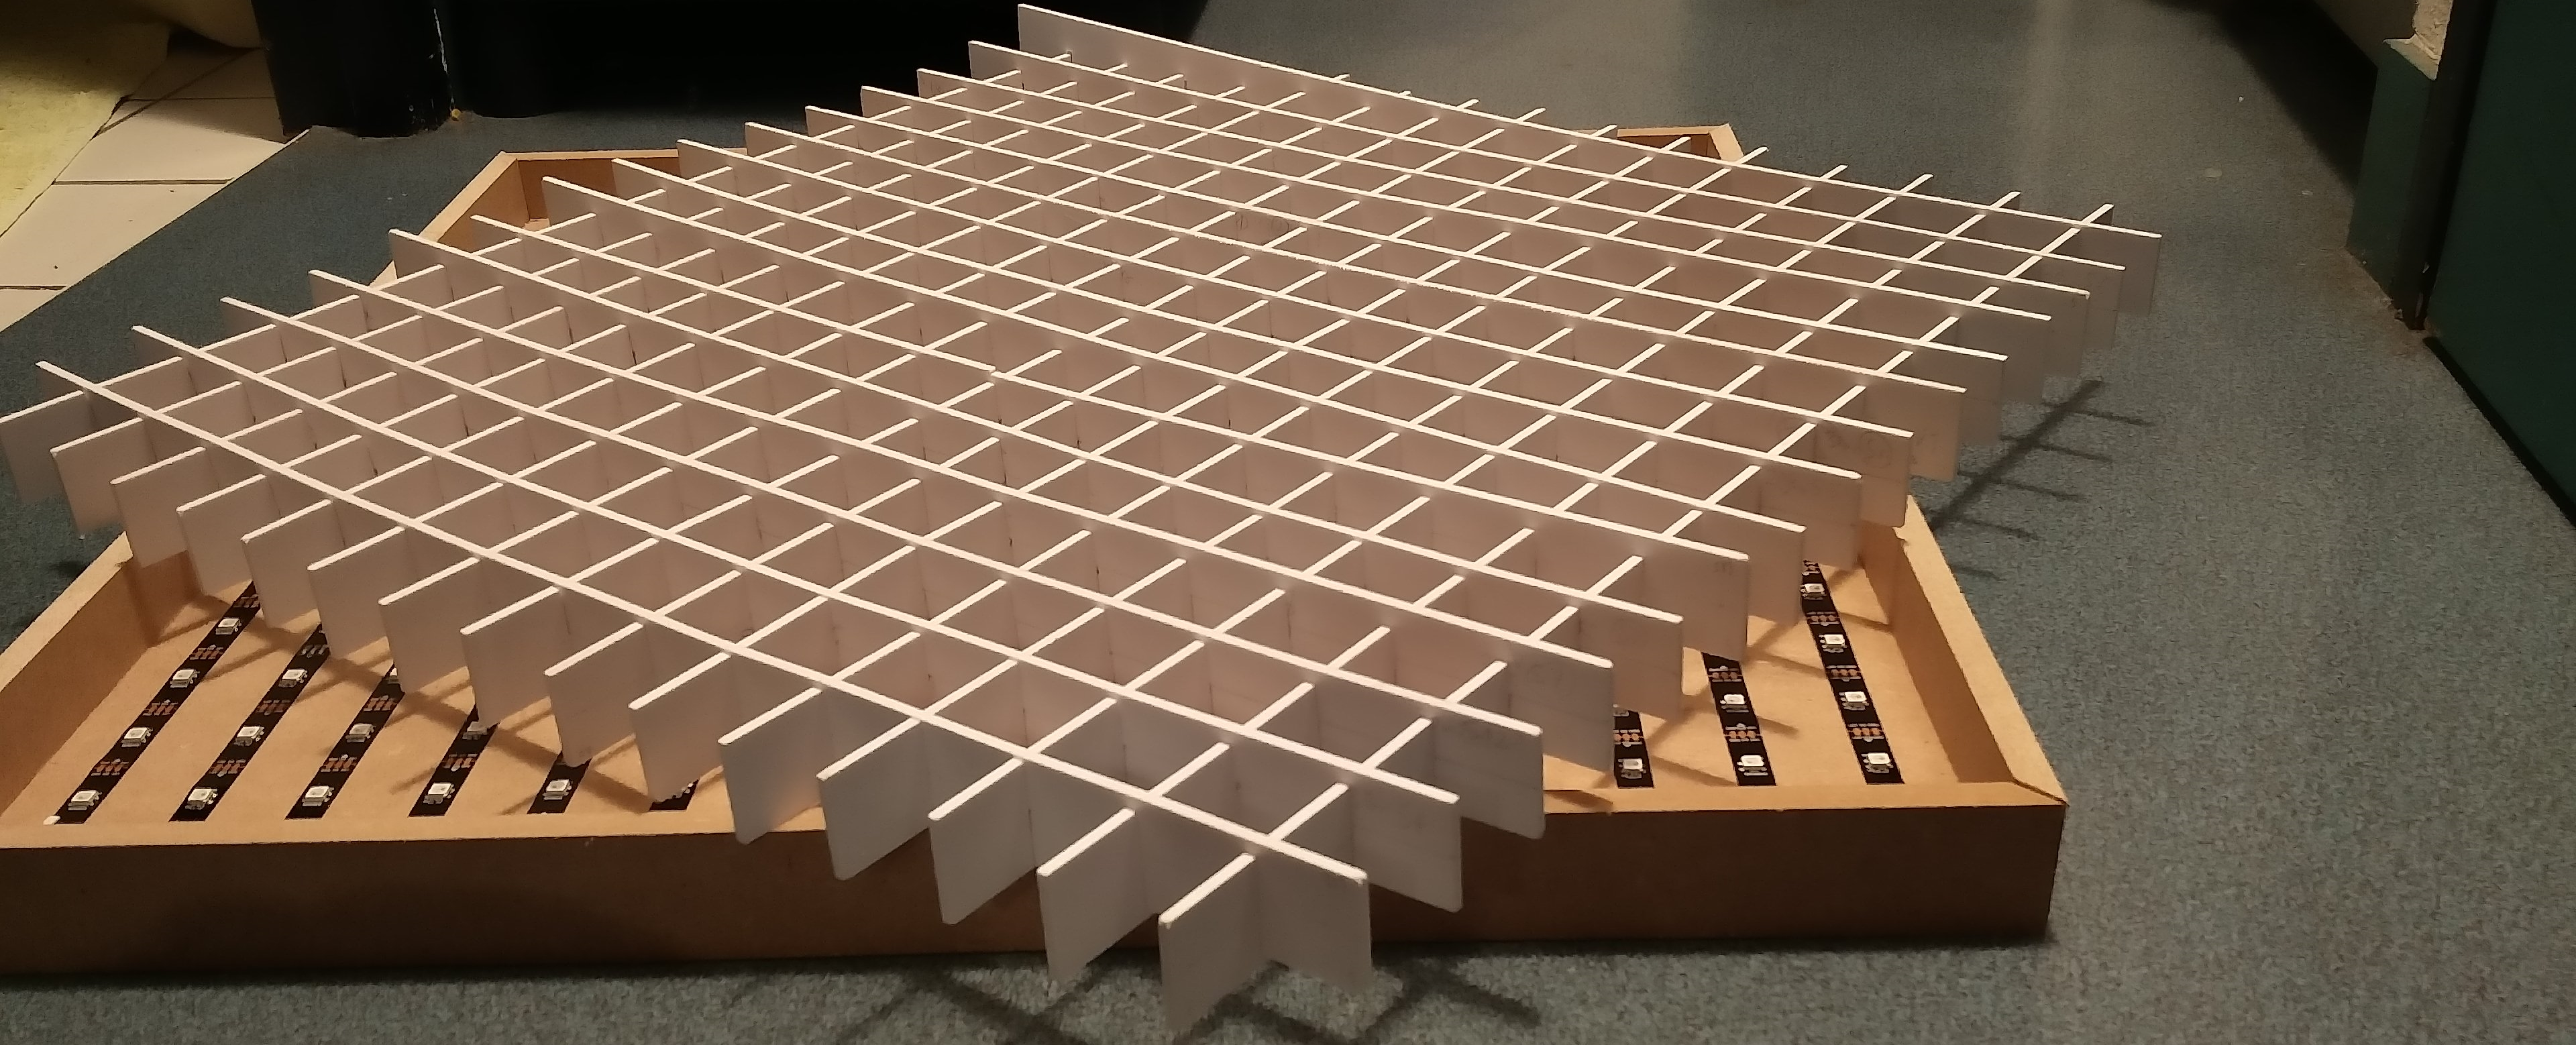
\includegraphics[width=\textwidth]{img/pic2}
\end{figure}\\
Due to the light intensity, we decided to put a 3mm transparent PVC layer at the top. Furthermore, we also put opaque PVC layers between each pixel.\\

The 16 LED strips (including 16 LEDs each) are linked in a ``snake'' layout to transmit the data signal all along BamboozLED\textsuperscript{TM}. The data signal is extended towards the Arduino driving the LED panel.

\subsection{Software}
In order to control the animation running on BamboozLED\textsuperscript{TM}, we used Glediator \cite{glediator}: this software offers several possibilities through its interface: pictures mixing, colors effects\ldots~The greatest feature of Glediator is the ability to modify how the signal is trasmitted to the Arduino depending of the layout of the target panel (we can specify panel dimensions, we can use a set of several panels, etc.).
\begin{figure}[htbp]
	\centering
	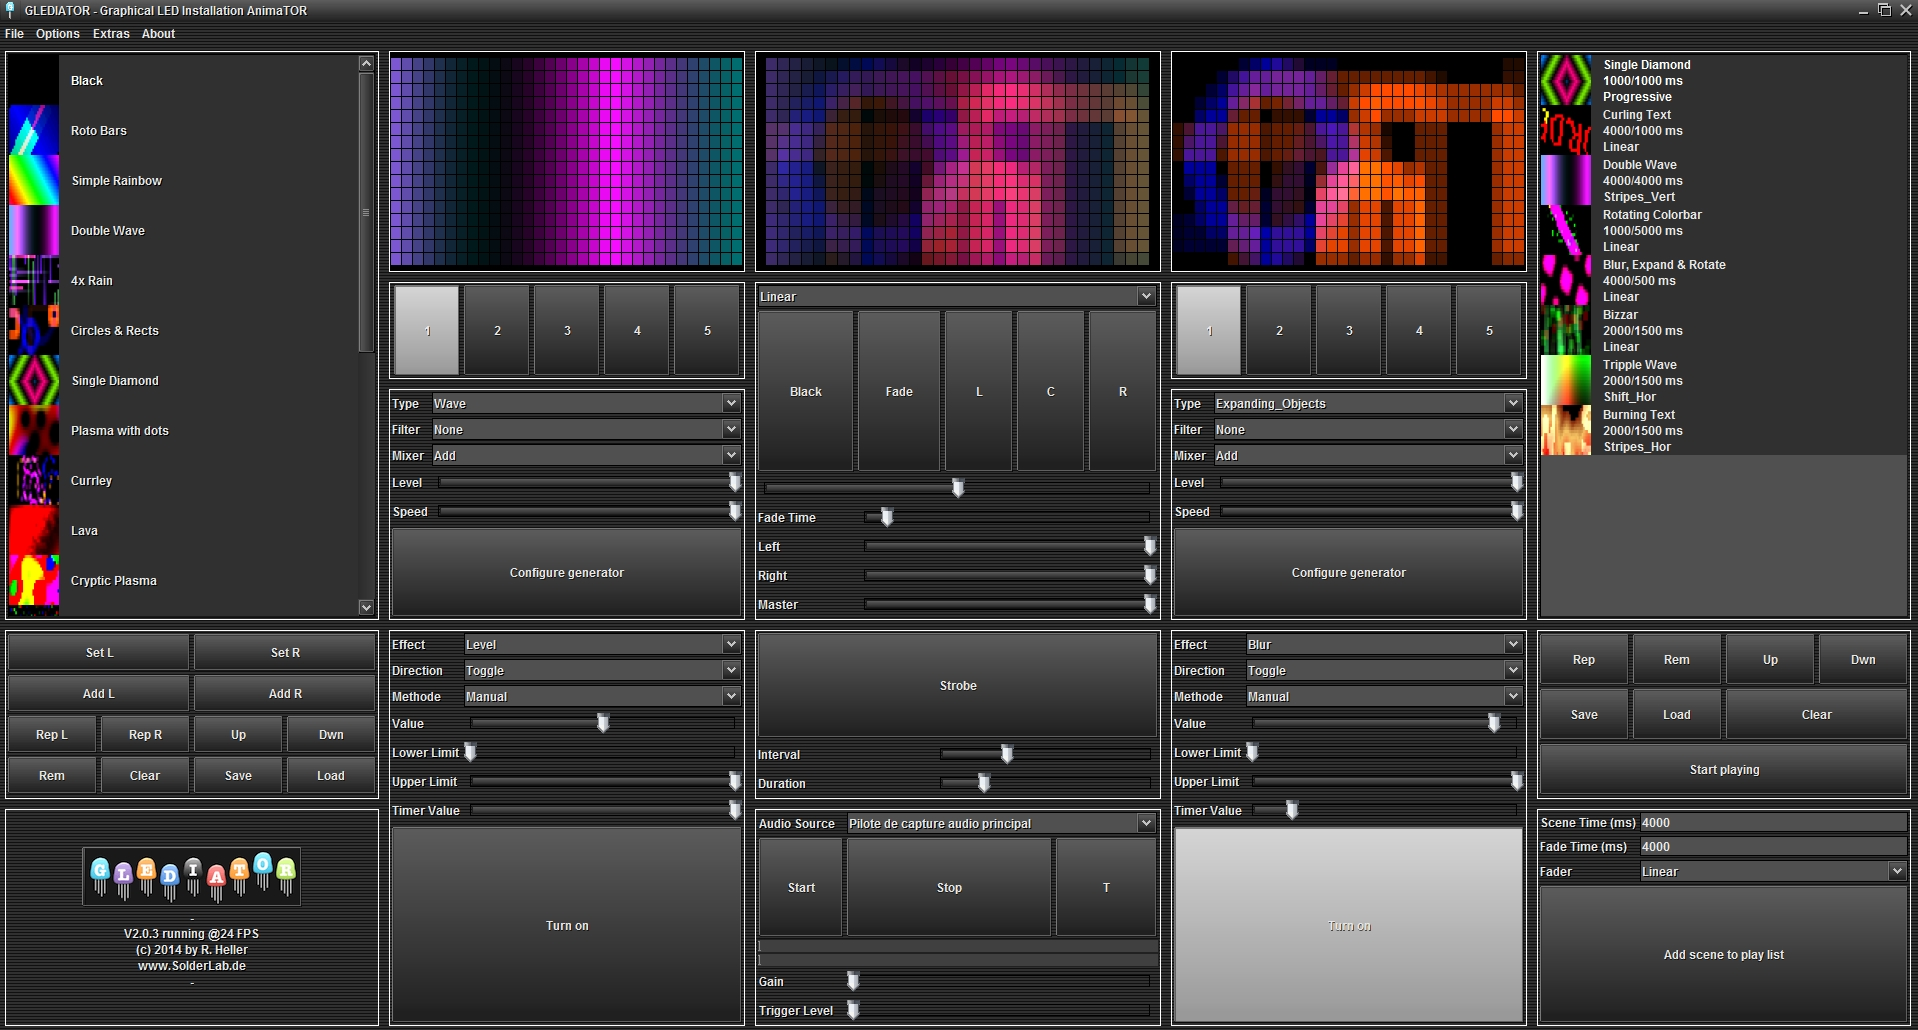
\includegraphics[width=\textwidth]{img/glediator}
\end{figure}

\section{Conclusion}
BamboozLED\textsuperscript{TM} is finally a low-cost RGB LED panel that can be used as a geeky decoration or as a f***** great screen for student parties. For BamboozLED\textsuperscript{TM} v2.0, we plan to create several panels which can be associated and more or less automatically detected by the microcontroller driving the whole circuit. Basically, something like Aurora \cite{aurora} but much cheaper!
\newpage
\bibliographystyle{ieeetran}
\bibliography{biblio}
\end{document}